% -------------------------------------------------------------------------
\begin{frame}{SYCL}
% \begin{center}
SYCL is a \textbf{parallel focused} abstraction layer created for C++

Characteristics:
\begin{columns}
  \begin{column}{0.48\textwidth}
    \begin{itemize}
      \item High-level
      \item Standard and modern C++
      \item Single source
      \item Portable code \\~\\
    \end{itemize}
  \end{column}
  \begin{column}{0.48\textwidth}
    \begin{center}
      
\includegraphics[width=0.7\linewidth]{Images/sycl-logo.png}
    \end{center}
  \end{column}
\end{columns}
\block{}
\begin{center}
  Targets a range of heterogeneous devices and backends
\end{center}
\endblock{}
\end{frame}
% -------------------------------------------------------------------------
\begin{frame}{SYCL}
\begin{center}
\begin{figure}[H]
  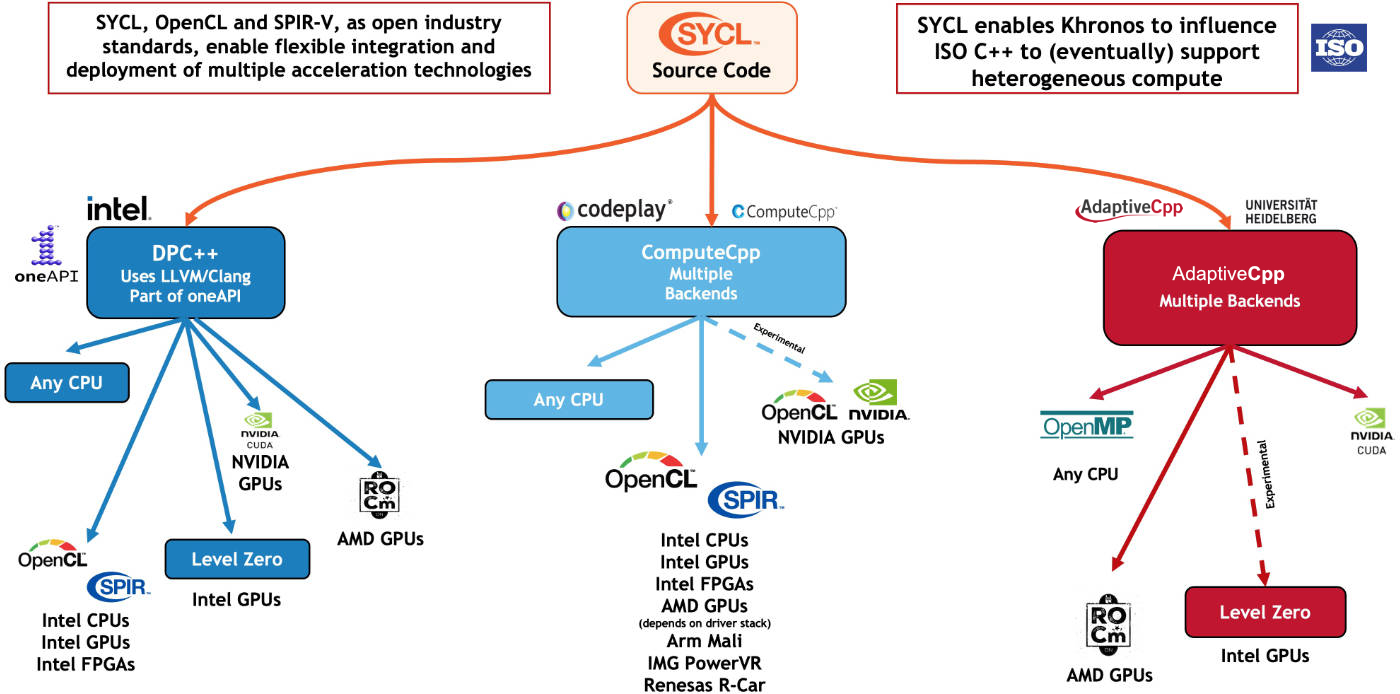
\includegraphics[width=\linewidth]{Images/sycl-map.png}
\end{figure}
SYCL backends map. \textit{(Credit: \url{www.khronos.org})}
\end{center}
\end{frame}
% -------------------------------------------------------------------------
\begin{frame}{SYCL}
  SYCL learning resources used:
\begin{columns}
  \begin{column}{0.48\textwidth}
    \begin{center}
    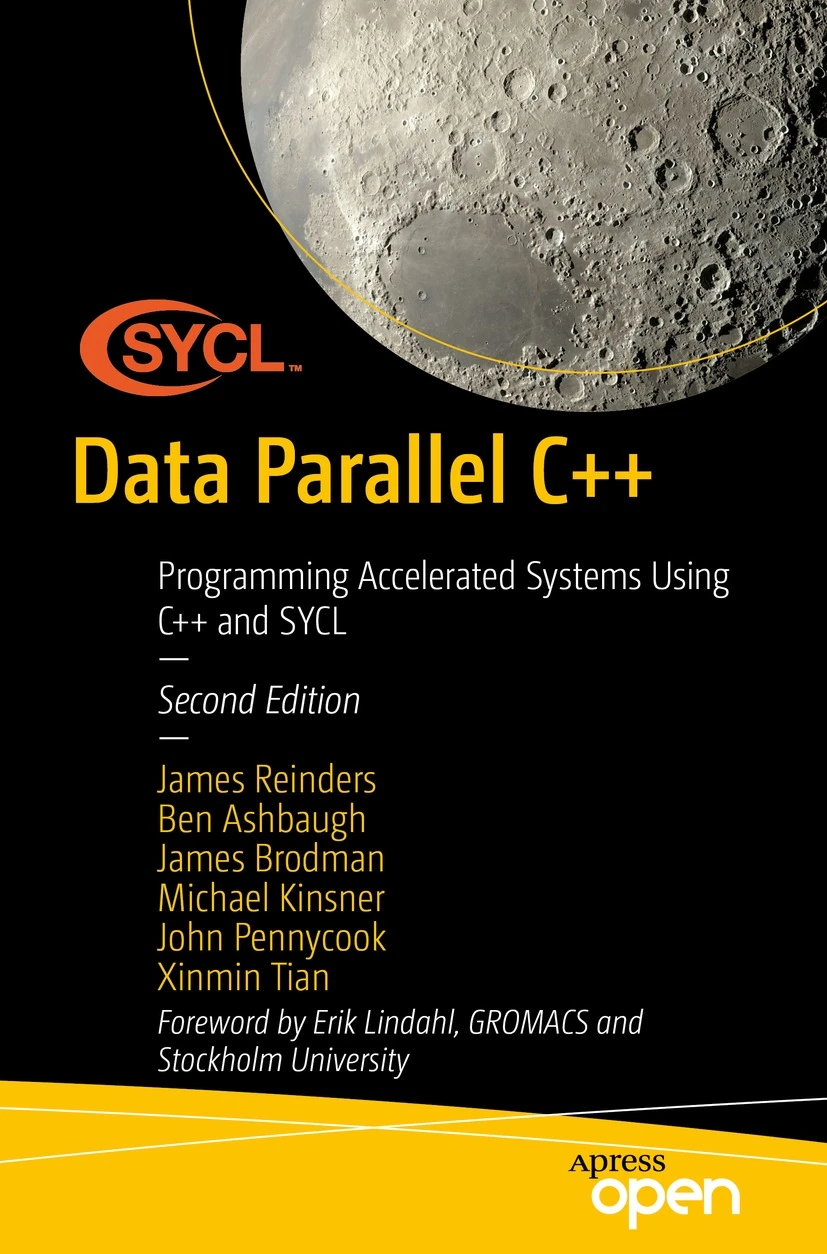
\includegraphics[width=0.6\linewidth]{Images/data-parallel-cpp.png}

    Extensive book on SYCL
    \end{center}
  \end{column}
  \begin{column}{0.385\textwidth}
    \begin{center}
    
\includegraphics[width=0.7\linewidth]{Images/sycl-academy.png}
    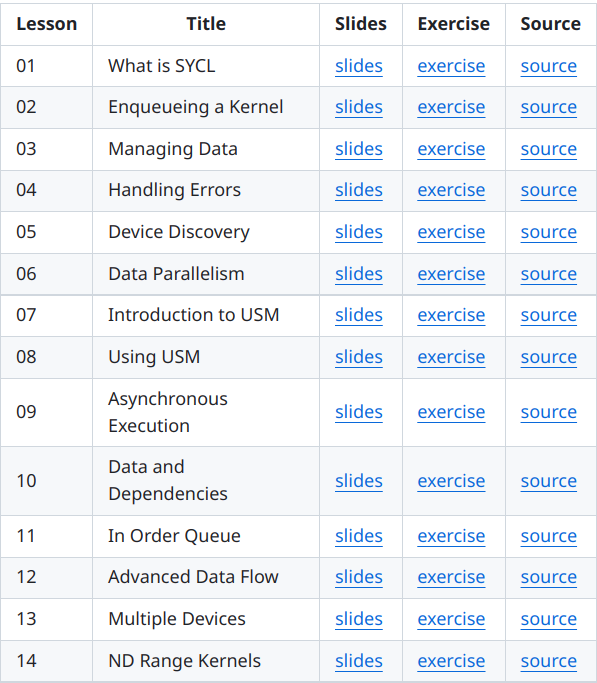
\includegraphics[width=0.9\linewidth]{Images/lessons.png}

    Practical tutorial lessons
    \end{center}
  \end{column}
\end{columns}
\end{frame}
% -------------------------------------------------------------------------
\begin{frame}{SYCL}
\begin{columns}
  \begin{column}{0.7\textwidth}
    \centering
  \lstinputlisting[language=C++,style=cppstyle]{Code/scalar_add.cc}
Scalar add. \href{{https://github.com/AdrianoMoreira08/TFG-SYCL/blob/main/sycl-examples/scalar_add.cc}}{\textit{See on Github}}
\end{column}
\begin{column}{0.3\textwidth}
  \begin{enumerate}
    \item Queue creation
    \item Buffer definition
    \item Command Group
    \begin{enumerate}
      \item Accessors
      \item Kernel
    \end{enumerate}
\end{enumerate}
\end{column}
\end{columns}
\end{frame}
% -------------------------------------------------------------------------
\begin{frame}{SYCL}
  \begin{figure}[H]
  \centering
  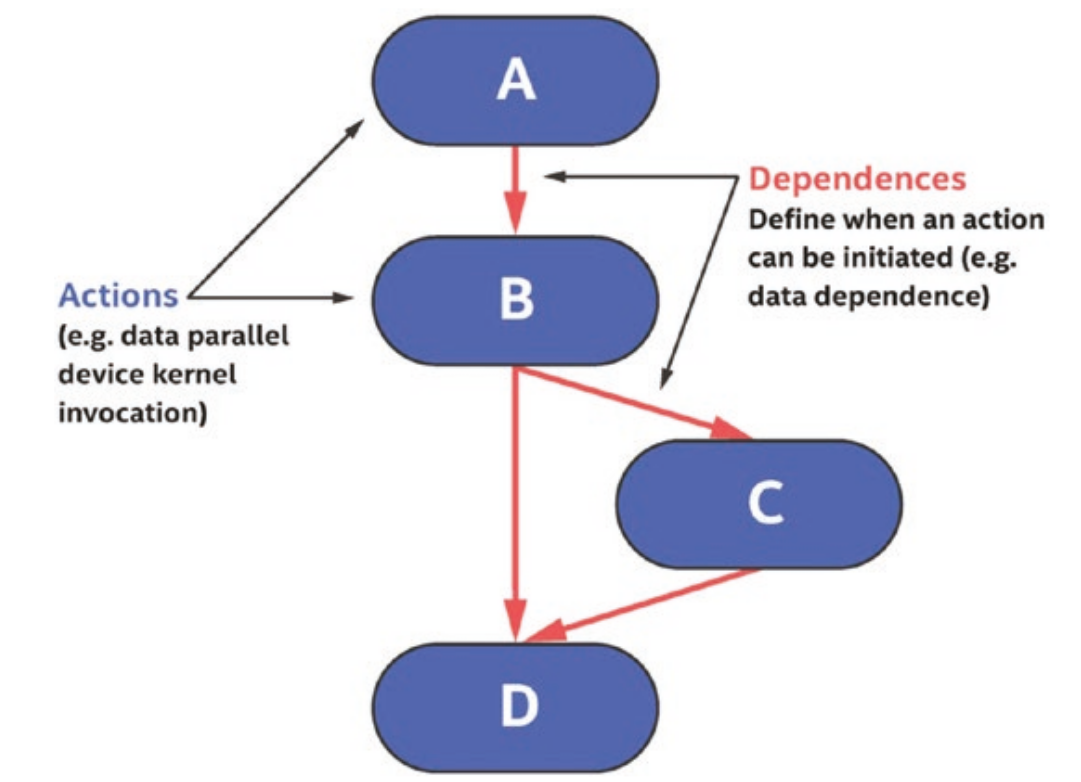
\includegraphics[width=0.74\linewidth]{Images/dependency-graph.png}

  Dependency graph example. \textit{Image From Data Parallel C++}
\end{figure}
\end{frame}
% -------------------------------------------------------------------------
\begin{frame}{SYCL}
  \begin{columns}
    \begin{column}{0.7\textwidth}
      \centering
    \lstinputlisting[language=C++,style=cppstyle]{Code/scalar_add.cc}
  Scalar add. \href{{https://github.com/AdrianoMoreira08/TFG-SYCL/blob/main/sycl-examples/scalar_add.cc}}{\textit{See on Github}}
  \end{column}
  \begin{column}{0.3\textwidth}
    \begin{enumerate}
      \item Queue creation
      \item Buffer definition
      \item Command Group
      \begin{enumerate}
        \item Accessors
        \item Kernel
      \end{enumerate}
  \end{enumerate}
  \end{column}
  \end{columns}
  \end{frame}
  % -------------------------------------------------------------------------
\begin{frame}{SYCL}
  \begin{figure}[H]
    \centering
    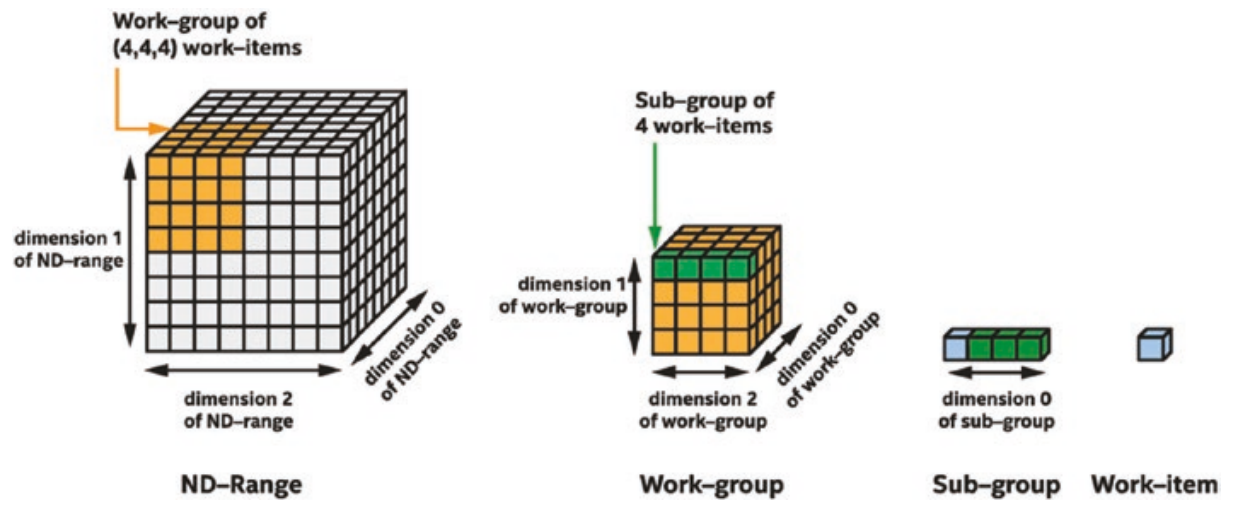
\includegraphics[width=\linewidth]{Images/nd_range.png}
    Dissection of an NDRange. \textit{From Data Parallel C++}
  \end{figure}
\end{frame}
